\documentclass[tikz,border=3.14mm]{standalone}

\begin{document}

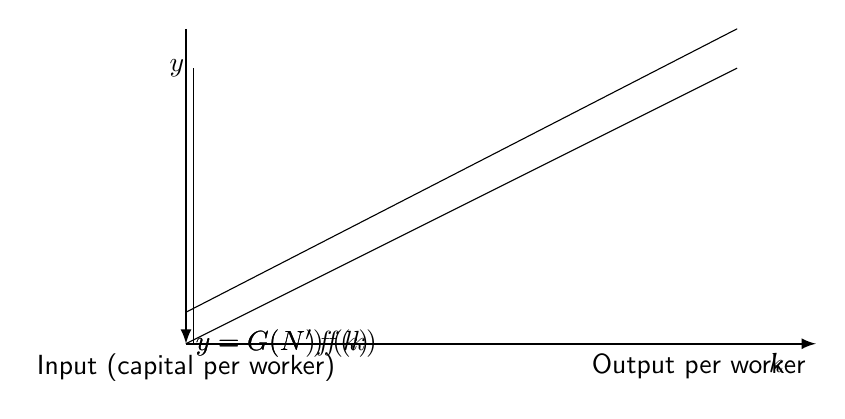
\begin{tikzpicture}[font=\sffamily]
    \draw[thick,-latex] (0,4) -- (0,0) node[below] {Input (capital per worker)};
    \draw[thick,-latex] (0,0) -- (8,0) node[below left] {Output per worker};
    \draw (0.1,3.5) node[left] {$y$} |- (7.5,0) node[below] {$k$};
    \draw (0,0) coordinate (O) edge (7,3.5) node[pos=0.9,right] {$y=G(N)f(k)$};
    \draw (0,0.4) edge (7,4) node[pos=0.9,right] {$y=G(N')f(k)$};
\end{tikzpicture}

\end{document}